\chapter[Chapter 9]{Chapter 9}\label{chap30}

\Authorline{M S Vidya\footnote[*]{Email: \url{vidya.m.rao@gmail.com}}}
\addtocontents{toc}{\protect\contentsline{section}{{\sl M S Vidya}\smallskip}{}}
\lhead[\small\thepage]{\small\leftmark}
\bigskip

There can be no two arguments about the importance of getting a good grip on one of the widely used mathematical tools in physics - vectors. The school definition of a vector as an entity endowed with the twin property of magnitude and direction in space has become an automated response to the question `what a vector is,' especially by students at the degree or post graduate level. This can only mean that the richness of the tool has not yet been appreciated or internalized. More so because the use of this tool lies scattered across many branches of physics and the necessary mathematical apparatus, perhaps, has not been acquired.

From the vantage position he had, Professor G Ramachandran  (GR to all of us) saw how easily these ideas could be brought within the reach of students - even school and junior college students. And he did just this in his monograph: \textit{Introduction to Vectors, Axial Vectors, Tensors and Spinors}\footnote[1]{G Ramachandran, M S Vidya and Venkataraya, Introduction to Vectors, Axial Vectors, Tensors and Spinors (Vijayalakshmi Prakashana, 2017).}. For courageous, serious minded students desirous of working on their backlogs or for those willing to gallop ahead  to unravel for themselves the intricacies of the subject, the monograph is a treat. Especially Chapter 9, for here the rewards are reaped.  After amassing the many gems  - ideas, notations and subtleties - strewn along in the initial chapters, the reader happily sees them come together in Chapter 9 to create a grand initiation to quantum theory.  And what of Chapter 10, the culminating chapter? It may appear to end the monograph abruptly - with no concluding remarks; but by then one realizes that any abruptness in a journey is just a short pause to consolidate the gains and move on; as one must.
\newpage

That GR had, to his share, a lot more excitement than just authoring and seeing through the publication of this monograph is evident from his selection of a quote for it; which he considered as much applicable to himself as to Issac Newton. And I suppose to each one of us:

{\quote{I do not know what I may appear to the world, but to myself I seem to have been only like a boy playing on the seashore, and diverting myself in now and then finding a smoother pebble or a prettier shell than ordinary, whilst the great ocean of truth lay all undiscovered before me. - \textit{Isaac Newton}}}
\vspace{1cm}

\drawline
\bigskip
\bigskip

\centerline{\includegraphics[scale=1.2]{authorsphotos/M_S_Vidya.eps}} 
\medskip

\noindent
{\biofntsize\textbf{Dr.\ M. S. Vidya} obtained M.Sc.\ in 1986 and the Ph.D. degree in 1998 from Mysore University. She worked for Ph.D.  under the guidance of Prof.\ G. Ramachandran. She worked as Lecturer in Physics from 1986 to 1992, first at Shree Jayachamarajendra College of Engineering and then at Yuvaraja College, Mysore. She was the Coordinator of the Science Centre at Mysore during 1992 to 1996. She was a Fellow of Vigyan Prasar, New Delhi, during 1998--99. She is the Founder Trustee of Vidya Online Charitable Trust, New Delhi. Currently she is leading an active retired life in Mysuru.}
